\section{Introduction}

Midsurface is an abstraction for thin-walled portions. Shell elements, based on midsurface, will give sufficiently close analysis results compared to that of 3D Solid elements. 'Thin Wall' is an inherent characteristic of the Sheet Metal parts and thus this work will cater to features prominent in Sheet Metal CAD applications. Midsurface can be used in thin portions of usual/mixed-dimensional/thick-thin parts also, but there, one needs to work out treatment of interfaces/joints/couplings which is considered out-of-scope for the current research. Midsurface is expected to have proper connectivity  (no gaps) and it should follow shape of the base part. As midsurface is generated Face-Pair wise, it needs to be stitched together to form a continuous shape. In midsurfacing techniques there are two broad categories namely, 'Medial Axis Transform (MAT)' and 'Midsurface Abstraction(MA)'.

	\begin{figure}[h]
	\centering
	\includegraphics[width=0.8\linewidth]{../Common/images//MAT_Midsurf.png}
	\caption{Midsurface Extration Methods}
	\label{MATMidsurf}
	\end{figure}
	
	
%	\begin{wrapfigure}{l}{0.62\textwidth}
%	\begin{center}
%	\includegraphics[scale=0.6]{images//MAT_Midsurf.png}
%	\end{center}
%	\caption{Midsurface Extration Methods}
%	\label{MATMidsurf}
%	\end{wrapfigure}
MAT is locus of the center of an inscribed disc of maximal diameter as it rolls around the object interior. The associated radius function gives radius of the inscribed circle at every point on the skeleton, and makes the original 2D object recoverable from the medial axis. In 2D its called Medial Axis Curve (Figure \ref{MATMidsurf}) where as in 3D it is called Medial Surface. Major drawback of this method is that it creates unnecessary branches and its shape is smaller than the original corresponding faces. Plus there is major issue of perturbations, meaning slight change in the base geometry forces re-computation of MAT and the result could very well be different than the original. 

MA (Figure \ref{MATMidsurf}) involves constructing 3D mid-surface for a part model by connecting/sewing the mid-surface patches obtained from each of the 'pairs of surfaces'. This requires a 'pairing strategy' that has thus far required human intervention in non-trivial cases. Connecting various mid-surface patches requires 3D non-manifold boolean operations. The surface-pairing approach has benefits over MAT techniques because the resultant geometry is cleaner and requires less reconstruction. However the surface pairing approach also has problems because it can be difficult to identify all of the surface pairs. Typically the idealization offered by the commercial programs is poor, and does not accurately represent the geometry they are idealizing\cite{Robinson2006}. Instead of basing the construction on the information contained in the feature model, the geometry as a whole is analyzed and then a global abstracted shape is derived, commonly based on the medial surface, medial axis, or a similar skeletal structure.  In this process, however, the connection of the analysis geometry with the features, the corresponding semantics, and the constraints that define the design model, is lost \cite{Smit2011}.

Both the above mentioned techniques are based on extraction where algorithm is applied on the final share. Many a times, due to complexity in recognizing forms, and due to complex interactions between them, midsurface of the part does not follow its form and is not fully connected \cite{Jxcad,Sheen2008} . Solution could be, to create midsurface while building the model itself.

In Features-based Solid Modeling, input feature-parameters are used to build tool-bodies and the whole part gets built using direct or indirect boolean of base and tool bodies. Creating midsurface for individual tool bodies appears to be a more deterministic problem than recognizing the feature forms. With well-defined boolean operations, correct midsurface connectivity can be ensured.  To the best of author's knowledge and during the literature review done so far, such system was not found either in the academic research or in the commercial applications.

%=================================================================================================================

\section{Related Work}

Good amount of research has been done in both approaches MAT and MA, but for different application domains. Midsurface is commercially available in many CAD/CAE packages. What's lacking in them is the usage of feature information. Various reasons for not using the feature-information are access-restrictions to the proprietary feature information, unsuitable non-manifold structure, as well as impracticality to include CAE structures in CAD software. There has been some work using M-Rep (Medial Representation similar to B-rep) which uses Medial entities as data model. But it has very basic data model and is mainly for medical visualization and not in the domain of Feature-based Modelers\cite{Thall2004}. Another related effort generates mid-curves in sketch and then sweeps to form midsurface \cite{Robinson2006}. This work is in Mix-Dimensional modeling, limited to sweep and does not seem to do feature interactions. 

Lee et al. suggested a conversion method from a sheet model to a solid model for the efficient solid modeling of thin-walled plastic or sheet metal parts. This method shows a great potential for degenerate solids in the representation of thin-walled parts. However, because this method adopts non-manifold boundary representation, it is difficult to represent
the exact adjacency relations between topological entities in a sheet model and to describe a mixture of wire and sheet objects that appear in the intermediate steps of sheet modeling operations. In order to overcome these problems, Lee et al. \cite{Lee2001} introduced a non-manifold boundary representation as a topological framework and proposed
a sheet thickening algorithm by presenting variations to a general non-manifold offset algorithm that is based on the mathematical definition of offsets. In addition, to facilitate sheet-modeling operations,  they provided a set of generalized Euler operators for non-manifold models as well as sheet modeling capabilities including adding, bending, and punching functions with two-dimensional curve editors. However, in these algorithms, all of the holes that lay
on thickness faces cannot be removed automatically and topological irregularity of an offset face caused by self-intersection is not yet considered \cite{Lee2001}.


Thus research so far does not deal with the major problems of midsurface, that of connectivity and simplification. Gaps and extraneous features in midsurface render it useless for meshing operation. Proposed research is planning for improved and robust generation and connectivity of midsurface\cite{Sheen2008}.


